\documentclass[11pt,a4paper]{article}
\usepackage[latin1]{inputenc}
\usepackage[margin=1in]{geometry}
\usepackage{amsmath}
\usepackage{amsfonts}
\usepackage{amssymb}
\usepackage{graphicx}
\usepackage{enumitem}
\usepackage{listings}
\usepackage{color}

\definecolor{dkgreen}{rgb}{0,0.6,0}
\definecolor{gray}{rgb}{0.5,0.5,0.5}
\definecolor{mauve}{rgb}{0.58,0,0.82}

\lstset{frame=tb,
 language=MatLab,
 aboveskip=3mm,
 belowskip=3mm,
 showstringspaces=false,
 columns=flexible,
 basicstyle={\small\ttfamily},
 numbers=none,
 numberstyle=\tiny\color{gray},
 keywordstyle=\color{blue},
 commentstyle=\color{dkgreen},
 stringstyle=\color{mauve},
 breaklines=true,
 breakatwhitespace=true,
 tabsize=3
}

\setlength\abovedisplayskip{0pt}
\author{James Brissette}
\title{CS-6210: HW 3}
\begin{document}
	\maketitle
	
	\section{Chapter 5}
		\begin{itemize}
			\item[5.10]
				\begin{enumerate} [label={\alph*)}]
					\item We can see for $J_0(x) = \frac{1}{\pi}\int_{0}^{\pi}cos(xsinx)ds$ that $\vertJ_0(x)\vert \leq 1$ by noting that the behavior of cosine is such that it is bounded between -1 and 1. This means that the absolute value of cosine will always be less than or equal to 1, and if we apply this to the integral then we can see that $\int_{0}^{\pi}cos(xsinx)ds \leq \int_{0}^{\pi}\pi ds$ and that is visible in the following plot:
					\begin{center}
						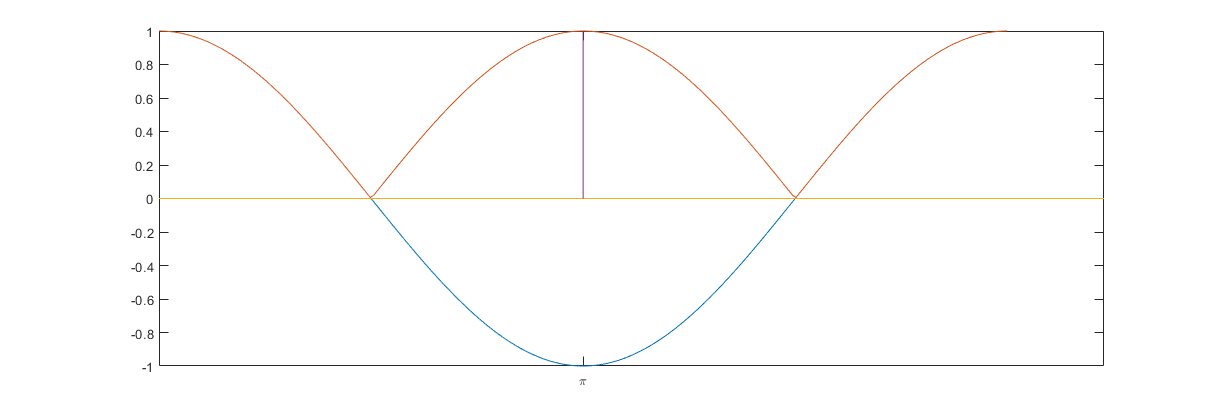
\includegraphics[width=1\linewidth]{ch5q10}
					\end{center}
				where $\int_{0}^{\pi}\pi ds$ is the area of the upper left rectangle. The area of $\frac{1}{\pi}\int_{0}^{\pi}cos(xsinx)ds \leq \frac{1}{\pi}\int_{0}^{\pi}\pi ds = \frac{\pi}{\pi} = 1$ \\
				
				We can extend this idea by noting that the derivatives of sin and cos are sin and cos, and so each subsequent derivative of each will yield a function who shares the same property of being bounded between -1 and 1, and the same logic follows for $\vertJ'_0(x)\vert$, $\vertJ''_0(x)\vert$, and so on.
					\item From Theorem 5.4 we see that $\vert f(x) - g(x) \vert \leq \frac{1}{8}h^2\vert \vert f'' \vert \vert_\infty$ and from part a we show that each subsequent derivative will be less than or equal to 1, so $\vert \vert f'' \vert \vert_\infty = max_{a \leq x \leq b} \vert f''(x) \vert = 1$. Using this to solve for $h$, we see that 
					$$\frac{1}{8}h^2 \leq 10e-06$$
					$$h \leq \sqrt{8*10e-06}$$
					and we have that the interval under consideration is $0 \leq x \leq 10$ so we can relate $h$ and $n$ as follows:
					$$h = 10/(n-1) \rightarrow n = \frac{10}{h}$$
					$$n \geq \frac{10}{\sqrt{8*10e-06}} + 1$$
					$$n \geq 1.119033e+03$$
					
					\item From Theorem 5.5 we follow the same logic for $\vert \vert f'''' \vert \vert_\infty$ and the error statement thus reads $\vert f(x)-s(x) \vert \leq \frac{5}{384}h^4 \leq 10e-06$, solving for $h$ we see:
					$$h = \sqrt[4]{\frac{384*10e-06}{5}}$$
					$$n \geq \frac{10}{\sqrt[4]{\frac{384*10e-06}{5}}} + 1$$
					$$n \geq 6.107029e+01$$
					\item From Theorem 5.8 we have $\vert f(x) - p_n(x) \vert \leq \frac{1}{2^n(n+1)!}(\frac{b-a}{2})^{n+1}\vert \vert f^{n+1} \vert \vert_\infty$. Using the same logic as before we deduce $\vert \vert f^{n+1} \vert \vert_\infty = 1$ and solving for $n$ we see:
					$$ \frac{1}{2^n(n+1)!}(\frac{10}{2})^{n+1} \leq 10e-06 $$
					Using Matlab to solve for $n$, we see that this equality holds when $n \geq 13$
					\item Because the Bessel function for higher orders follows the same logic as for lower orders, and because the new variable introduced is with respect to the differentiation variable $ds$, we know that when we integrate it will go away, and so there is no change from the argument introduced in part a, and our answers don't change for parts b through d.
				\end{enumerate}
					
			\item[5.11]
				\begin{enumerate} [label={\alph*)}]
					\item For $g(x)$ to be a cubic spline, the following basic conditions must be met:
					$$\begin{array}{cc}
						g_1(x_1)=y1 & g_1(x_2)=y2 \\
						g_2(x_2)=y2 & g_2(x_3)=y3 
					\end{array}$$~
					$$\begin{array}{c}
						g'_1(x_2)=g'_2(x_2)\\
						g''_1(x_2)=g''_2(x_2)
					\end{array}$$
					In an attempt to find the relationship between $\alpha$ and $\beta$, and in order to deduce the values that make $g'_1(x_2)=g'_2(x_2)$ true, we equate the derivatives of $g_1$ and $g_2$ and we see that @ $x=0$ this is true for all values of $\alpha$ and $\beta$:
					$$6x+3\alpha x^2=2 \beta x + 3x^2 \rightarrow \quad true \quad \forall \alpha,\beta \quad @x=0$$
					Taking the second derivatives we see that for $6+6\alpha x = 2 \beta + 6x$ that at the point where the two curves meet ($x=0$), we get $2\beta = 6$ or $\beta = 3$. Again here we see that the we're not constrained to a specific value of $\alpha$. As an aside, interestingly enough if you plug $\beta = 3$ back into the first derivatives and set them equal to each as we did before, you find that $\alpha = -1$ for every value of x where $x\neq0$ and plugging that $\alpha$ and $\beta$ into $g_1$ and $g_2$ you see that they're equivalent for all values of x:
					$$g_1 = 2+3x^2 -x^3 \quad @\alpha=-1$$
					$$g_2 = 2+3x^2 -x^3 \quad @\beta=3$$
					
					\item Taking $\beta = 3$ we have points $(1,4)$,$(0,2)$ and if we assume $\alpha=-1$, (-1,6). If we don't make that assumption, we have $(-1,5-\alpha)$
					\item We can find the value for which $g(x)$ is a natural cubic spline by setting the second derivatives of $g_1$ and $g_2$ at the endpoints to 0 and solving for $\alpha$ and $\beta$:
					$$\begin{array}{ccc}
					s_1''(-1) = 0 & & s_2''(+1) = 0 \\
					6+6\alpha x = 0 & & 2\beta - 6x = 0 \\
					6\alpha=6 & & \beta = 3 \\
					\alpha=1 & &
					\end{array}$$
					\item We can find the value for which $g(x)$ is a clamped cubic spline by setting the first derivatives of $g_1$ and $g_2$ equal to $y'$ at the endpoints and solving for $\alpha$ and $\beta$. However, since we don't have a distinct value for $\alpha$ from part a, we can't find an exact solution:
					$$\begin{array}{ccccc}
					s_1'(-1) & = & 6x + 3\alpha x^2& = & y'_{-1} \\
					s_1'(-1) & = & -6 + 3\alpha & = & y'_{-1} \\
					 & & \alpha & = & (y'_{-1} + 6)/3 \\
					  & & & & \\
					s_2'(1) & = & 2 \beta x - 3 x^2& = & y'_{+1} \\
					s_2'(1) & = & 2 \beta- 3 & = & y'_{+1} \\
					& & 3 & = & y'_{+1}
					\end{array}$$
				\end{enumerate}
				
			\item[5.15]
				\begin{enumerate} [label={\alph*)}]
					\item Fitting the data with a global polynomial using Lagrange interpolation, and a natural cubic spline:
					\begin{center}
						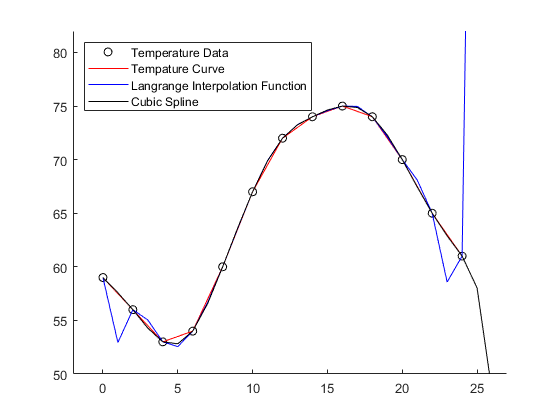
\includegraphics[width=1\linewidth]{ch5q15}
					\end{center}
				The code was all self-written and is located at the end of this file.\\
				
					\item At 11 AM the two interpolation functions give the following:
					$$\begin{array}{ccc} 
					Lagrange & & Natural Cubic Spline \\
					6.9913129e+01 & & 6.9881177e+01 \\
					69.9^{\circ} & & 69.8^{\circ}
					\end{array} $$
					\item At 1 AM the next day the two interpolation functions give the following:
					$$\begin{array}{ccc} 
					Lagrange & & Natural Cubic Spline \\
					1.5204891e+02 & & 5.8029609e+01 \\
					152.05^{\circ} & & 58.03^{\circ}
					\end{array} $$
					\item At 9 AM the next day the sun hides it face for shame at the blazing temperature Lagrange has unleashed upon the world:
					$$\begin{array}{ccc} 
					Lagrange & & Natural Cubic Spline \\
					4.5226229e+05 & & 0 \\
					452,262.29^{\circ} & & 0^{\circ}
					\end{array} $$
					Fun fact, this is about 1.8x hotter than the dead star at the center of the Red Spider Nebula $(\approx 250,000^{\circ})$ which itself is 25 times hotter than the surface of the sun. Here, however, we see that the cubic does not take a proportional dive to extreme lows and we can interpret this to show how Lagrange has a tendency to diverge drastically at the endpoints. The cubic dips down, yes, but handles the boundaries much better than the global interpolation polynomial using Lagrange.
				\end{enumerate}
				
			\item[5.22]
				\begin{enumerate} [label={\alph*)}]
					\item Looking first at Lagrange interpolation, we know that the polynomial $p_n(x)$ is a summation as follows:
					$$p_n(x) = \Sigma_{i=1}^{n+1} yi\ell_i(x), \quad where \quad \ell_i= \prod_{j=1,i \neq j}^{n+1} \frac{x-x_j}{x_i - x_j}$$
					In the formation of the Lagrange coefficient we see the numerator and denominator separated by one division, and both consisting of $n$ subtractions and ($n-1$) multiplications. Taking these together, we have 2($n+n-1$)+1 = $4n-1$ FLOPS for every Lagrange Coefficient. These calculated coefficients are then multiplied by the value $y_i$ (add 1), and this is done $n+1$ times (multiply by $n+1$). From this we have $(4n-1+1)(n+1)$. Lastly, each of the those terms is the summed, for a total of $n$ additions. This gives us $(4n^2+4n)+(n) = 4n^2+5n$. \\
					
					Looking next at the piece-wise linear interpolation, we have:
					$$G_i(x) = G(\frac{x-x_i}{h}) \quad where \quad G(x) = \begin{cases}
					1-\vert x \vert \quad if \quad \vert x \vert \leq 1 \\
					\mkern9mu 0 \quad \quad \quad if \quad 1 \leq \vert x \vert
					\end{cases}$$
					and we are solving for
					$$g(x) = \Sigma_{i=1}^{n+1} y_iG_i(x) $$
					As seen above, calculating $y_iG_i(x)$ takes 4 FLOPS (2 to evaluate $\frac{x-x_i}{h}$, 1 to evaluate $1-\vert x \vert$, and 1 to multiply $y_iG_i(x)$), and this is done $n+1$ times, after which each term is summed for a total of $n$ additions. We have $4(n+1)+n = 5n+4$ total FLOPS. \\
					
					Lastly, looking at the cubic spline interpolation, we have several parts to consider. The equation to solve takes the form:
					$$s(x) = \Sigma_{i=0}^{n+2}\mkern9mu a_iB_i(x)$$
					If we start by looking at the $B_i$'s we see that we need at most 8 FLOPS where each $B_i(x)$ is solved as follows:
					$$B_i(x) = B(\frac{x-x_i}{h}) \quad where \quad B(x) = \begin{cases}
					\mkern9mu \frac{2}{3} - x^2(1-\frac{1}{2}\vert x \vert)\quad if \quad \vert x \vert \leq 1 \\
					\mkern9mu \frac{1}{6}(2-\vert x \vert)^3 \quad \quad \quad \mkern9mu  if \quad 1 \leq \vert x \vert \leq 2 \\
					\mkern9mu 0 \quad \quad \quad \quad \quad \quad \quad \mkern9mu  if \quad 2 \leq \vert x \vert
					\end{cases}$$
					We count 2 to solve for $\frac{x-x_i}{h}$, and 6 to solve for $\frac{2}{3} - x^2(1-\frac{1}{2}\vert x \vert)$). We use this one instead of $\frac{1}{6}(2-\vert x \vert)^3$ because we see that when we evaluate a $x$ the highest FLOP count will come from the first statement.\\
					Now that we have the the $B_i$'s, we solve for the $a_i$'s which requires considerably more steps. To solve for the $n+3$ coefficients necessary, we will assume we already have the $n-1$ by $n-1$ tridiagonal matrix A, we need an 1 by $n-1$ vector $z$ and we need to evaluate a few $a_i$'s ($a_0$ and $a_{n+2}$) by hand. First, $a_0$ and $a_{n+2}$ require 2 FLOPS each to calculate $a_0 = 2a_1-a_2$, and $a_{n+2} = 2a_{n+1}-a_{n}$ for 4 total. Next, $z$ is formed by making $n-1$ multiplications (every element has a component that is multiplied by 6) and two subtractions at the first and last elements for $n+1$ FLOPS. \\
					
					Once these values are found, the Thomas algorithm solves for the remaining $a_i$'s in 8n-7 FLOPS. Putting it all together, we have (4)+(n+1)+(8n-7) = $9n-2$ FLOPS and fortunately we only have to calculate the $a_i$'s once. Returning to our equation for $s(x)$ we have that we calculate the value of the $a_i$'s once for $9n-2$ FLOPS, we then have 8 FLOPS to calculate $B_i$ and 1 multiplication for $a_iB_i(x)$. This is done $n+3$ times and then the values are summed for a total of $n+2$ additions:
					$$(9n-2)+(n+3)(9)+(n+2) = 19n+27$$
					
					From greatest to least we have Lagrange, cubic, piece-wise linear.
					
					\item From the last part we see that we only have to calculate the $a_i$'s once for the cubic spline, but we will have to calculate the Lagrange coefficients again for the new value of x (meaning the total FLOP count will not change), and we will need to again calculate the values of $G_i(x)$ for the piece-wise interpolation. Since Lagrange doesn't come down, and the cubic doesn't reduce significantly enough to beat the $5n+4$ FLOPS of the piece-wise, the ordering doesn't change, despite having pre-computed the $a_i$'s (making the cubic take at least $9n-2$ less FLOPS).
				\end{enumerate}
				
			\item[5.26]
				\begin{enumerate} [label={\alph*)}]
					\item If we determine the global interpolation polynomial using Lagrange interpolations, then we can see that given these data points, the Lagrange coefficients become:
					$$\ell_1 = \frac{(x-x_2)(x-x_3)(x-x_4)}{(x_1-x_2)(x_1-x_3)(x_1-x_4)}$$
					$$\ell_2 = \frac{(x-x_1)(x-x_3)(x-x_4)}{(x_2-x_1)(x_2-x_3)(x_2-x_4)}$$
					$$\ell_3 = \frac{(x-x_1)(x-x_2)(x-x_4)}{(x_3-x_1)(x_3-x_2)(x_3-x_4)}$$
					$$\ell_4 = \frac{(x-x_1)(x-x_2)(x-x_3)}{(x_4-x_1)(x_4-x_2)(x_4-x_3)}$$
					Solving for each we see the coefficients become $\ell = [0.3125,0.9375,-0.3125,0.0625]$ and interpolation polynomial returns:
					$$p_3=y_1\ell_1 + y_2\ell_2 + y_3\ell_3 + y_4\ell_4$$ $$= (0*0.3125) + (1*0.9375) + (0*-0.3125) + (1*0.0625) = 1$$
    
    				\item To find the natural cubic spline, we need to find the $a_i$'s and $B_i(x)$'s in the following equation:
    				$$s(x) = a_0B_0(x) + a_1B_1(x) + a_2B_2(x) + a_3B_3(x) + a_4B_4(x) + a_5B_5(x)$$
    				where 
    				$$B_i(x) = B(\frac{x-x_i}{h}) \quad where \quad B(x) = \begin{cases}
					\mkern9mu \frac{2}{3} - x^2(1-\frac{1}{2}\vert x \vert)\quad if \quad \vert x \vert \leq 1 \\
					\mkern9mu \frac{1}{6}(2-\vert x \vert)^3 \quad \quad \quad \mkern9mu  if \quad 1 \leq \vert x \vert \leq 2 \\
					\mkern9mu 0 \quad \quad \quad \quad \quad \quad \quad \mkern9mu  if \quad 2 \leq \vert x \vert
					\end{cases}$$
					We calculate:
					$$\begin{array}{ccccc}
					B_0(\frac{1}{2}) &=& \frac{1}{6}(2-\frac{3}{2})^3&=&0.0208\\
						B_1(\frac{1}{2}) &=& \frac{2}{3}-(\frac{1}{2}^2)(1-\frac{1}{2}*\frac{1}{2})&=&0.4792\\
						B_2(\frac{1}{2}) &=& \frac{2}{3}-(\frac{1}{2}^2)(1-\frac{1}{2}*\frac{1}{2})&=&0.4792\\
						B_3(\frac{1}{2}) &=& \frac{1}{6}(2-\frac{3}{2})^3&=&0.0208\\
						B_4(\frac{1}{2}) &=& 0&&\\
						B_5(\frac{1}{2}) &=& 0&&
					\end{array}$$
					Next, solving for the $a_i$'s, we see:
					$$\begin{array}{ccccc}
						a_1 & = & y_1 & = & 0\\
						a_4 & = & y_4 & = & 1
					\end{array}$$
					and we also know that in the general case:
					$$a_{i-1}+4a_i+a_{i+1}=6y_{i}$$
					so
					$$a_{1}+4a_{2}+a_{3}=6y_{2} \rightarrow a_2 = \frac{6-a_3}{4}$$
					$$a_{2}+4a_{3}+a_{4}=6y_{3} \rightarrow a_3 = \frac{1-a_2}{4}$$
					Solving these two equations gives us
					$$\begin{array}{ccc}
						a_2 & = & \frac{5}{3}\\
						a_3 & = & -\frac{2}{3}
					\end{array}$$
					and with these we can solve for the last two $a_i$'s
					$$\begin{array}{ccccc}
						a_0 & = & 2a_1 - a_2 & = & -\frac{5}{3}\\
						a_5 & = & 2a_4 - a_3 & = & \frac{8}{3}
					\end{array}$$
				Plugging all of these values back into $s(x)$ we get:
				$$s(.5) = -\frac{5}{3}*0.0208 + 0*0.4792 + \frac{5}{3}*0.4792 + -\frac{2}{3}*0.0208 + 1*0 + \frac{8}{3}*0$$
				$$s(.5) = .7500 $$
				\item The reason these two methods give us different answers is easiest to visualize in a plot:
					\begin{center}
						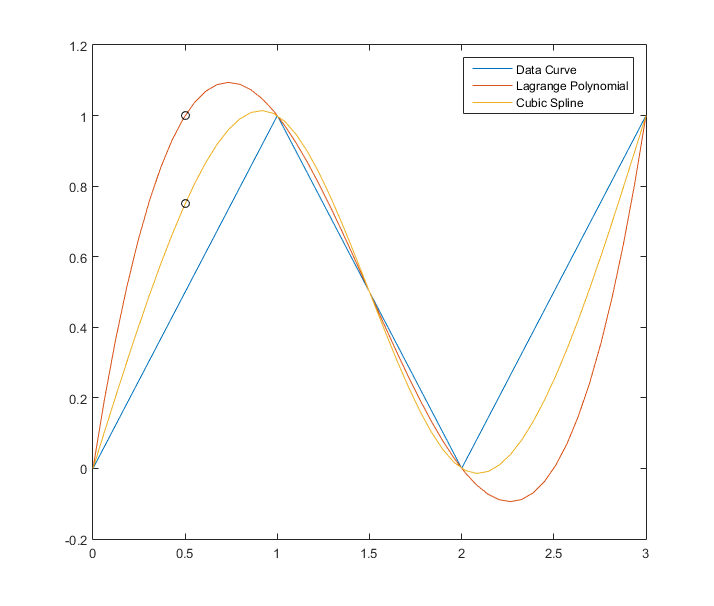
\includegraphics[width=1\linewidth]{ch5q26}
					\end{center}
					As we would imagine and as is the case with the Lagrange polynomial (and Vandermonde), the polynomial itself appears to oscillate more towards the boundaries and appears more fully consistent in the middle. Because of this, as the the global polynomial approaches the interpolation point at $x_2$ it swings higher and passes through (.5,1) where the spline more tightly fits the data. While both cubics are fully consistent with the data, the spline has a constraint that the global polynomial is not subject to, namely that $s''(x_1) = 0$ and $s''(x_n) = 0$, which is why both are consistent with the data but produce different results.
					\item As above, because we're imposing different constraints on the two functions, they produce different results. However, if we were to impose the constraint that the values of $s'$ at the boundaries matched the slope of y', we would have the same constraints and same polynomial. This has a convenient name in the case of cubic splines and is referred to as a 'clamped' cubic spline.
				\end{enumerate}
				
			\item[5.27]
				\begin{enumerate} [label={\alph*)}]
					\item We know that if the exact value of $cos(\frac{\pi}{k})$ (and sin) is known (for m=1), that we can use the following trigonometric identities to prove the rest are known by induction:
					$$cos(\alpha + \beta) = cos(\alpha)cos(\beta)-sin(\alpha)sin(\beta)$$
					$$sin(\alpha + \beta) = sin(\alpha)cos(\beta)+cos(\alpha)sin(\beta)$$
					If we know $cos(\frac{\pi}{k})$, then we can rewrite $cos(\frac{2\pi}{k})$ as cosine of $\frac{\pi}{k}$ + some multiple of $\frac{\pi}{k}$, like $cos(\frac{\pi}{k}+\frac{\pi}{k})$ and $sin(\frac{2\pi}{k})$ as sine of $sin(\frac{\pi}{k}+\frac{\pi}{k})$. This creates combinations of sines and cosines of factors that we stated are known. By following this pattern one notices:
					$$
					\begin{array}{ccc}
						cos(\frac{\pi}{k}) & = & a \\
						sin(\frac{\pi}{k}) & = & b \\
						cos(\frac{2\pi}{k}) & = & cos(\frac{\pi}{k})cos(\frac{\pi}{k})-sin(\frac{\pi}{k})sin(\frac{\pi}{k}) \\
						sin(\frac{2\pi}{k}) & = & sin(\frac{\pi}{k})cos(\frac{\pi}{k})+cos(\frac{\pi}{k})sin(\frac{\pi}{k}) \\
						cos(\frac{3\pi}{k}) & = & cos(\frac{\pi}{k})cos(\frac{2\pi}{k})-sin(\frac{\pi}{k})sin(\frac{2\pi}{k}) \\
						sin(\frac{3\pi}{k}) & = & sin(\frac{\pi}{k})cos(\frac{2\pi}{k})+cos(\frac{\pi}{k})sin(\frac{2\pi}{k}) \\
						 & \vdots & \\
						 cos(\frac{m\pi}{k}) & = & cos(\frac{\pi}{k})cos(\frac{(m-1)\pi}{k})-sin(\frac{\pi}{k})sin(\frac{(m-1)\pi}{k}) \quad for \mkern9mu m = 2,3,4\dots  \\
						sin(\frac{m\pi}{k}) & = & sin(\frac{\pi}{k})cos(\frac{(m-1)\pi}{k})+cos(\frac{\pi}{k})sin(\frac{(m-1)\pi}{k}) \quad for  \mkern9mu m = 2,3,4\dots
					\end{array}
					$$
					\item Given that we known $h=\frac{pi}{k}$ and that $h$ is the step size which is given by $h=\frac{x_n-x_1}{n-1}$, since it's given that the domain in from 0 to $2\pi$ we have the following:
					$$h=\frac{x_n-x_1}{n-1}=>\frac{2\pi}{n-1}=\frac{\pi}{k}$$
					$$n=2k+1$$
					\item Theorem 5.4 gives us that $\vert f(x)-g(x)\vert\leq \frac{1}{8}h^2\vert\vert f''\vert\vert_\infty$, and we know that $f''$ of $cos(x)$ is $-cos(x)$, and since cosine is bounded between -1 and 1, then the term $\vert\vert f'' \vert\vert_\infty = max_{a \leq x \leq b}\vert -cos(x) \vert = 1$. We want the error $\vert f(x)-g(x)\vert \leq \frac{1}{8}h^2 \leq 10^{-6}$ so we solve for $h$ and find that this is true when $h\leq \sqrt{8*10^{-6}}$, meaning the smallest value of $k$ for which this is still true is $k\geq \frac{\pi}{h}, \quad k\geq 3.5124e+02$.
					\item According to Theorem 5.5,  $\vert f(x)-s(x)\vert\leq \frac{5}{384}h^4\vert\vert f''''\vert\vert_\infty$, and we know that $f'$ of $cos(x)$ is $-sin(x)$, $f''$ of $cos(x)$ is $-cos(x)$, and $f'''$ of $cos(x)$ is $sin(x)$, so $f''''$ of $cos(x)$ is $cos(x)$. Since cosine is bounded between -1 and 1 then the term $\vert\vert f'''' \vert\vert_\infty = max_{a \leq x \leq b}\vert cos(x) \vert = 1$. Again we want the error $\vert f(x)-s(x)\vert \leq \frac{5}{384}h^4 \leq 10^{-6}$ so we solve for $h$ and find that this is true when $h\leq \sqrt[4]{384*10^{-6}/5}$ or $h\leq 1.6647e-01$, meaning the smallest value of $k$ for which this is still true is $k\geq \frac{\pi}{h}, \quad k\geq 1.8872e+01$.
					\item Given the sequence of calculating the exact values of sin and cosine, we could use a procedure that uses this induction logic to construct n values of $cos(\frac{m\pi}{k})$ for $m=2,3,4\dots n$. Additionally, we could use the results from parts c and d and deduce that a clamped cubic spline would be the ideal implementation. Part d tells us that the smallest value we could use for $k$ is 18, but the closest exact value of cosine is at $\frac{\pi}{20}$. Using our result from part b, at $k=20, n=41$. So our method should use multiples of $\frac{\pi}{20}$ to generate at least 41 points plotted with a clamped cubic spline.
					\item See below for the code used to generate the following chart. Note that the interpolation error for $x=1,2,5$ was $-1.1443e-06$, $3.3764e-07$, and $-9.8496e-08$ respectively.
					\begin{center}
						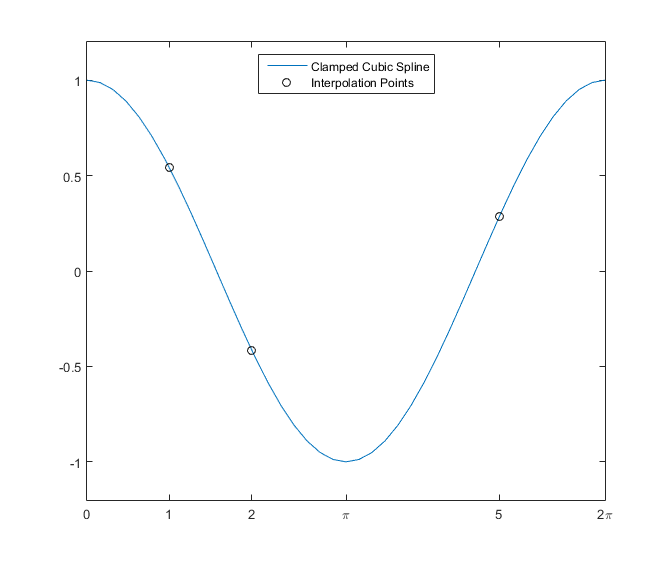
\includegraphics[width=1\linewidth]{ch5q27}
					\end{center}
				\end{enumerate}
				
			\item[5.28]
			
				\begin{enumerate} [label={\alph*)}]
					\item Since we have the data interval with respect to $x$ as $x_1\leq x \leq x_{n+1}$ and we have $z_i =\frac{x_i - \alpha}{\beta}$ then solving for $x_i$ we have $x_i = z_i\beta + \alpha$ and the interval with respect to $z$ is $z_1\beta+\alpha \leq z \leq z_{n+1}\beta + \alpha$. 
					\item In order to scale the data so that the z data interval is $-1 \leq z \leq 1$, we have that on the lower end $\frac{x_1-\alpha}{\beta}=-1$ and solving for $\alpha$ we see that $\alpha=\frac{\beta}{x_1}$. At the upper end of the range we have $\frac{x_{n+1}-\alpha}{\beta}=1$ and solving for $\beta$ we have that $\beta = x_{n+1}-\alpha$. Substituting $\beta$ into our equation for $\alpha$ we have:
					$$\alpha = \beta + x_1,\quad \beta = x_{n+1}-\alpha$$
					\begin{align*}
					\alpha &= x_{n+1}-\alpha + x_1 \\
					\alpha &= \frac{x_{n+1} + x_1}{2}
					\end{align*}
					\begin{align*}
					\beta &= x_{n+1}-\alpha \\
					\beta &= x_{n+1}-\frac{x_{n+1} + x_1}{2} \\
					\beta &= \frac{x_{n+1} - x_1}{2}
					\end{align*}
					
					\item See below for the plot of the direct approach using Vandermonde and the scaled method for part d. All code is below. Using the direct method, one finds the condition number of $V = 1.5929e+47$.
					\begin{center}
						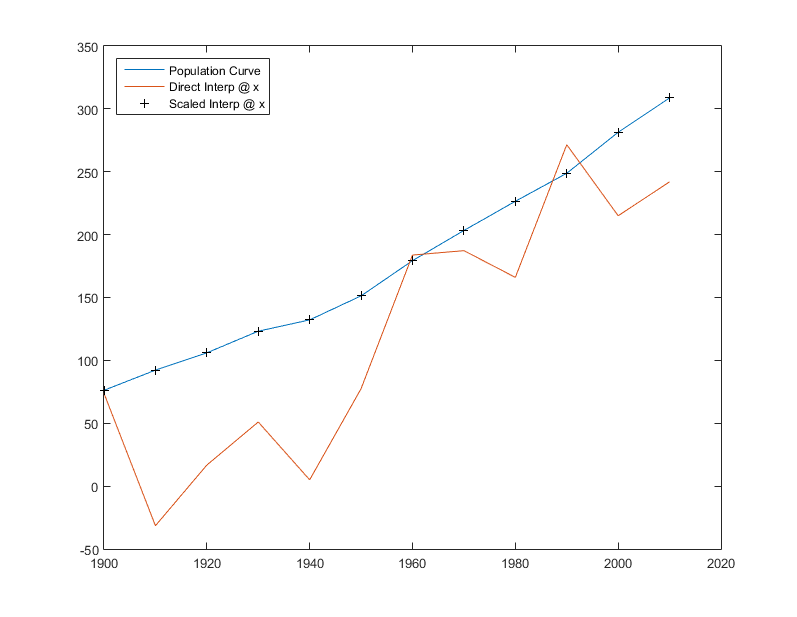
\includegraphics[width=1\linewidth]{ch5q28}
					\end{center}
					\item Using the $\alpha$ and $\beta$ computed in part b, I was able to find the coefficients and plot the new interpolation function in the plot above. The condition number using the scaled method was $4.075488e+04$ 
				\end{enumerate}
			
			\item[5.33]
				\begin{enumerate} [label={\alph*)}]
					\item Because we have $n$ functions, each of which have 3 coefficients, we need an equivalent number of constraints. The first condition $w_i(x_i) =y_i$ applies to all $n$ functions, as does $w_i(x_i+1)=y_{i+1}$. From these two conditions, we have $2n$ constraints. However, because we are equating the first derivatives of consecutive functions in the last constraint, $w'_{i}(x_{i+1}) = w'_{i+1}(x_{i+1})$, we \textit{would} only have $n-2$ functions for which the derivative is known, however, since the text explicitly states that we are given $b_1$ then we have $n-1$ consecutive functions the constraint applies to. In total we have $(2n)+(n-1)=3n-1$ constraints.\\
					
					Additionally, we are able to deduce that $b_1$ is the same as the slope of $w_1(x_1)$ in that the slope of $w_1(x_1)$ is equal $w'_1(x_1)$ and we know that this is equal to $b_1+2c_1(x-x_1)$ where $x=x_1$, meaning our $2cx$ term goes away and we are left with $w'_1(x_1)=b_1$.
					
					\item To show that $a_i=y_i for i=1,2,\dots,n+1$, we simply look at the value of $w_i(x_i)$ for any given value of $i$. For example we get 
					$$w_i(x_i)=a_i+b_i(x_i-x_i)+c_i(x_i-x_i)^2$$
					$$w_i(x_i)=a_i$$ 
					and from our constraint $w_i(x_i) =y_i$ we have that $$w_i(x_i) =a_i = y_i$$
					
					To show that $b = -b_{i-1}+2(y_i - y_{i-1} )/h$ it's easier to first show that $c_i = (y{i+1} - y_i - hb_i)/h^2$. To show this we observe use the fact that $a_i=y_i$ and use the condition that $w_i(x_i+1)=y_{i+1}$ by solving for $c_i$ when $x = x_{i+1}$:
					$$\begin{array}{ccccc}
						w_i(x_{i+1}) &=& a_i + b_i(x_{i+1}-x_i)+c_i(x_{i+1}-x_i)^2 &=& y_{i+1}\\
						w_i(x_{i+1}) &=& y_i + b_i(h)+c_i(h)^2 &=& y_{i+1} \\
						& & b_i(h)+c_i(h)^2 &=& y_{i+1}-y_i \\
						& & c_i &=& (y_{i+1}-y_i-hb_i)/h^2
					\end{array}$$
				
					Using this result we can substitute in to the derivative and leverage the constraint that $w'_{i}(x_{i+1}) = w'_{i+1}(x_{i+1})$ to find $b_i$. To simplify the expressions, we will previously assert that $w'_{i+1}(x_{i+1})=b_{i+1}+2c_{i+1}(x_{i+1}-x_{i+1})=b_{i+1}$:
					$$\begin{array}{ccccc}
						w'_i &=& b_i+2c_ih &=& b_{i+1}\\
						&&b_i&=& b_{i+1}-2c_ih \\
						&&b_i&=& b_{i+1}-2(\frac{y_{i+1}-y_i-hb_i}{h^2})h\\
						&&b_i&=& b_{i+1}-2(\frac{y_{i+1}-y_i}{h} - b_i) \\
						&&b_i&=& -b_{i+1}+2(\frac{y_{i+1}-y_i}{h}) \\
						&&b_{i-1}&=& -b_{i}+2(\frac{y_{i}-y_{i-1}}{h}) \\
						&&b_{i}&=& -b_{i-1}+2(\frac{y_{i}-y_{i-1}}{h})
					\end{array}$$
					
					\item Parts $a$ and $b$ indicate that you can solve for all of the coefficients for $w_i$ for all $i$ in that we learn the $a$ is tied to the value of $y$, so those are available at the outset since we start with $y$. It shows that $c_i$ depends on the value of $b_I$ and that $b_i$ depends on the value of $b_{i-1}$. Because we are given $b_1$ we can calculate $c_1$ and $b_2$, and since we now have $b_2$ we can calculate the value of $c_2$ and $b_3$ and so on.
					\item The interpolated values work fairly well for this function at larger values of n, but the function itself has a lot of strange behavior and so it's clear this particular function is difficult to interpolate. This is more pronounced when n is small. Code below.
					\begin{center}
						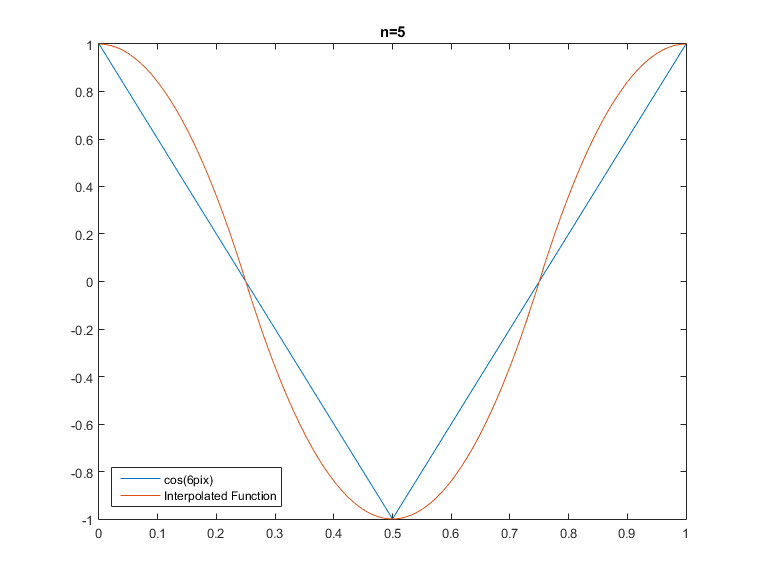
\includegraphics[width=1\linewidth]{ch5q33_5}
					\end{center}
					\begin{center}
						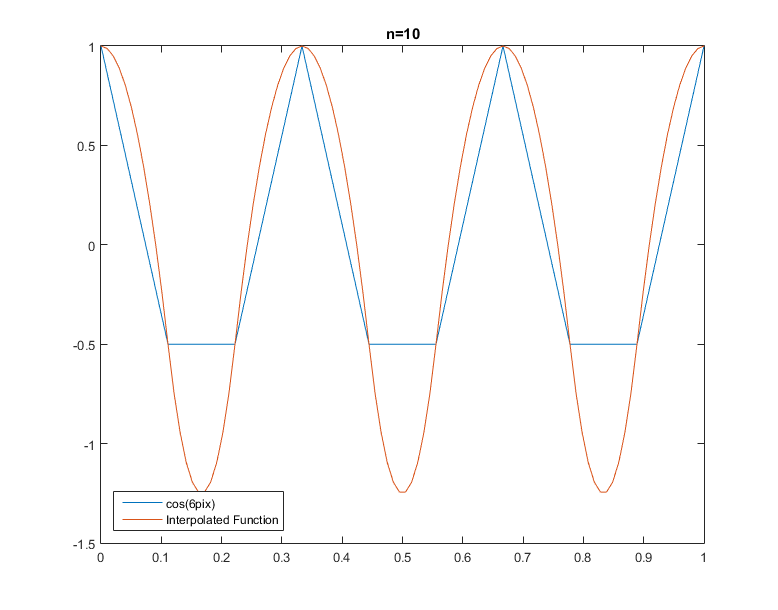
\includegraphics[width=1\linewidth]{ch5q33_10}
					\end{center}
					\begin{center}
						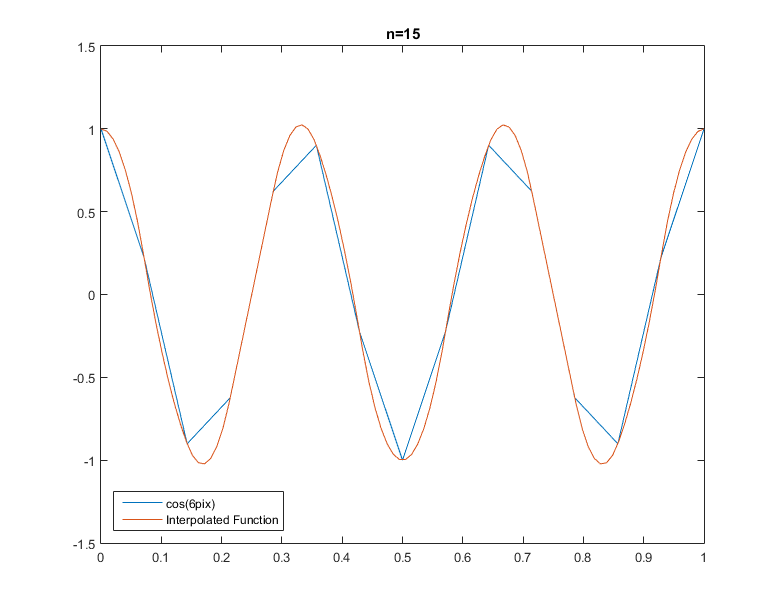
\includegraphics[width=1\linewidth]{ch5q33_15}
					\end{center}
					\begin{center}
						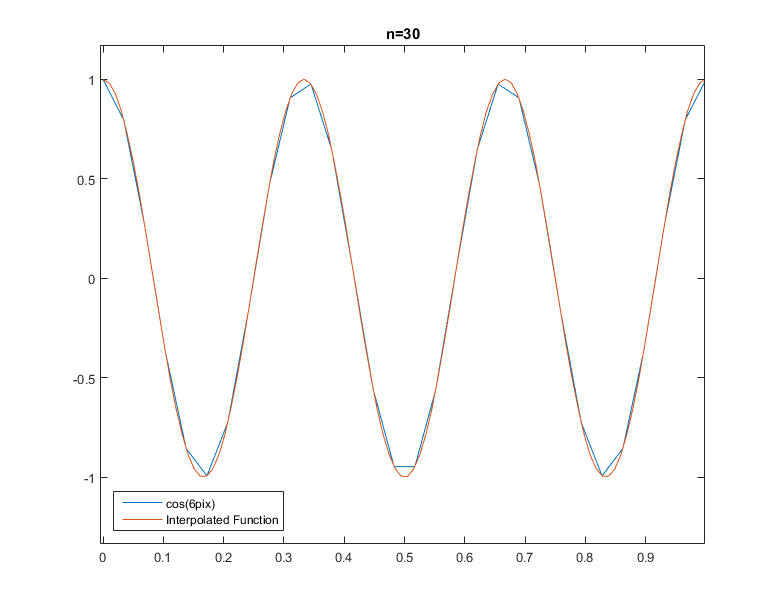
\includegraphics[width=1\linewidth]{ch5q33_30}
					\end{center}
				\end{enumerate}
		\end{itemize}
	\section{Code:}
	\begin{lstlisting} 
	function [ output ] = ch5q15()
	%ch5q15
	x = linspace(0,24,13);
	[m,n] = size(x);
	y = [59,56,53,54,60,67,72,74,75,74,70,65,61];
	
	nx = 25+9; %Adding 9 to evaluate at 9am the next day
	interpolationPoints = linspace(x(1),x(n)+9,nx);
	
	%p is the output using the interpolation polynomial
	p = zeros(nx,1);
	
	%Compute the Lagrange Polynomial
	for i = 1:nx
	px = 0;
	lagrangeCoefficient = ell(interpolationPoints(i),x);
	for j = 1:n
	px = px + y(j)*lagrangeCoefficient(j);
	end
	p(i) = px;
	end
	
	hold on
	
	output = zeros(nx,2);
	output(:,1) = p;
	scatter(x,y,'ko');
	plot(x,y,'r',interpolationPoints,p,'b');
	%The CubicSpline was handled seperately
	output(:,2) = CubicSpline(x,y,nx);
	hold off
	legend('Temperature Data','Tempature Curve','Langrange Interpolation Function','Cubic Spline','Location','northwest');
	axis([-2,27,50,82]);
	
	end
	\end{lstlisting}
	
	\begin{lstlisting}
	function [coefficients] = ell(interp, xs)
	%Computes the Lagrange Coefficients
	[m,n] = size(xs);
	coefficients = zeros(n,1);
	
	for i=1:n
	val = 1;
	for j=1:n;
	if (i == j)
	continue
	end
	val = val * (interp - xs(j)) / (xs(i)-xs(j));
	end
	coefficients(i) = val;
	end
	end
	\end{lstlisting}
	
	\begin{lstlisting}
	function [ output ] = CubicSpline(x,y,nx)
	
	h = x(2)-x(1);
	[m,n] = size(x);
	
	%s is the output using the cubic spline
	s = zeros(1,nx);
	interpolationPoints = linspace(x(1),x(n)+9,nx);
	
	n = n-1;
	B = zeros(1,n+3);
	
	%%%%Compute the Natural Cubic Spline
	% Calculate ai's
	A = tridiag(4,1,n-1);
	z = zeros(n-1,1);
	z(1) = 6*y(2)-y(1);
	z(n-1) = 6*y(n)-y(n+1);
	for k = 2:n-2
	z(k) = 6*y(k+1);
	end
	
	%a is incremented to reflect 1-indexing, not zero
	a = zeros(1,n+3);
	% a(1) & a(n+1)
	a(2) = y(1);
	a(n+2) = y(n+1);
	
	%  Solve for middle ai's using Thomas Algorithm
	a(3:n+1) = Thomas(A,z);
	
	%  a(0) & a(n+2)
	a(1) = 2*a(2)-a(3);
	a(n+3) = 2*a(n+2)-a(n+1);
	
	%new vector xx is the vector x with one additonal point at each end
	xx = zeros(n+3,1);
	xx(2:n+2) = x;
	xx(1) = xx(2)-h;
	xx(n+3) = xx(n+2)+h;
	
	for i = 1:nx
	val = 0;
	for j = 1:n+3
	%Calculate Bi
	cx = (interpolationPoints(i)-xx(j))/h;
	
	if (abs(cx) < 1)
	B(j) = (2/3)-(cx^2)*(1-(.5*abs(cx)));
	elseif (abs(cx) < 2)
	B(j) = ((2-abs(cx))^3)/6;
	else
	B(j) = 0;
	end
	
	val = val + a(j)*B(j);
	end
	s(i) = val;
	end
	
	output = s';
	plot(interpolationPoints,s,'k')
	hold off
	end
	
	
	\end{lstlisting}
	
	\begin{lstlisting}
	function [x] = Thomas(A,z)
	%Thomas Algorithm
	%   For solving tridiagonal matrices as given in Table 3.6
	[m,n] = size(A);
	x = zeros(n,1);
	v = zeros(n,1);
	w = A(1,1);
	x(1) = z(1)/w;
	
	for i = 2:n
	v(i) = A(i-1,i)/w;
	w = A(i,i)-A(i,i-1)*v(i);
	x(i) = (z(i)-A(i,i-1)*x(i-1))/w;
	end
	
	for j = (n-1):-1:1
	x(j) = x(j)-v(j+1)*x(j+1);
	end
	
	end
	\end{lstlisting}
	
	\begin{lstlisting}
	function [ output ] = tridiag(a,b,n)
	%Creates an nxn tridiagonal matrix with 'a' along the main diagonal
	
	output = zeros(n);
	output(1,1) = a;
	for i = 2:n
	output(i,i) = a;
	output(i-1,i) = b;
	output(i,i-1) = b;
	end          
	
	end
	\end{lstlisting}
	
	\begin{lstlisting}
	function [out] = Vandermonde(x)
	
	[m,n] = size(x);
	out = zeros(n);
	out(:,1) = 1;
	for i=2:n
	out(:,i) = x.^(i-1);
	end
	
	end
	\end{lstlisting}
	
	\begin{lstlisting}
	function [output] = ch5q27()

	h = pi/20;
	nx = 3;
	x = linspace(0,40*pi/20,41);
	[sinx,y] = cosPiTwenty(41);
	
	[m,n] = size(x);
	
	s = zeros(1,nx);
	interpolationPoints = [1,2,5];
	
	n = n-1;
	B = zeros(1,n+3);
	
	%%%%Compute the Clamped Cubic Spline
	% Calculate ai's
	A = tridiag(4,1,n-1);
	z = zeros(n-1,1);
	z(1) = 6*y(2)-y(1);
	z(n-1) = 6*y(n)-y(n+1);
	for k = 2:n-2
	    z(k) = 6*y(k+1);
	end
	
	%a is incremented to reflect 1-indexing, not zero
	a = zeros(1,n+3);
	% a(1) & a(n+1)
	a(2) = y(1);
	a(n+2) = y(n+1);
	%  Solve for middle ai's using Thomas Algorithm
	
	a(3:n+1) = Thomas(A,z);
	a(1) = -sinx(1)*2*h+a(3);
	a(n+3) = sinx(n+1)*2*h+a(n+1);
	
	xx = zeros(n+3,1);
	xx(2:n+2) = x;
	xx(1) = xx(2)-h;
	xx(n+3) = xx(n+2)+h;
	
	for i = 1:nx
	    val = 0;
	    for j = 1:n+3
	        cx = (interpolationPoints(i)-xx(j))/h;
	        if (abs(cx) < 1)
	            B(j) = (2/3)-(cx^2)*(1-(.5*abs(cx)));
	        elseif (abs(cx) < 2)
	            B(j) = ((2-abs(cx))^3)/6;
	        else
	            B(j) = 0;
	        end
	        val = val + a(j)*B(j);
	    end
	    s(i) = val;
	end
	
	output = s';
	
	plot(x,y);
	set(gca,'xtick',[0 1 2 pi 5 2*pi])
	set(gca,'xticklabel',{'0','1','2','\pi','5','2\pi'})
	axis([0,2*pi,-1.2,1.2]);
	hold on
	scatter(interpolationPoints,s,'k')
	legend('Clamped Cubic Spline','Interpolation Points','Location','North')
	
hold off
	end


	\end{lstlisting}
	\begin{lstlisting}
	function [s,c] = cosPiTwenty(nx)
	%Calculate the exact value of cos from 0 to nx*pi/20 in pi/20 steps

	c = ones(1,nx);
	s = zeros(1,nx);

	%start indexing at 2 so output = [0,pi/20,2pi/20,...]
	s(2) = (sqrt(2)*(sqrt(5)+1)-2*sqrt(5-sqrt(5)))/8;
	c(2) = (sqrt(2)*(sqrt(5)+1)+2*sqrt(5-sqrt(5)))/8;

	for i=2:nx-1
    	c(i+1) = c(2)*c(i)-s(2)*s(i);
   	 	s(i+1) = s(2)*c(i)+c(2)*s(i);
	end

	end
	\end{lstlisting}
	\begin{lstlisting}
	function [ output ] = ch5q28()
	%Part c/d
	
	x = linspace(1900,2010,12);
	y = [76.21,92.23,106.0,123.2,132.2,151.3,179.3,203.3,226.5,248.8,281.4,308.7];
	[m,n] = size(x);
	
	V = Vandermonde(x);
	fprintf('The condition number of V using the direct method is %d \n',cond(V));
	a = V\y(1:n)';
	output = a;
	
	%Calculating pn(xi) using Vandermonde Coefficients
	s = ones(n,2);
	s(:,1) = s(:,1)*a(1);
	for i = 1:n
	    for j = 2:n
	        s(i,1) = s(i,1) + a(j)*x(i)^(j-1);
	    end
	end
	
	%Calculating pn(zi) where each z is the corresponding scaled x value
	alpha = (x(n)+x(1))/2;
	beta = (x(n)-x(1))/2;
	z = (x-alpha)/beta;
	
	Vz = Vandermonde(z);
	fprintf('The condition number of V using the scaled method is %d \n',cond(Vz));
	az = Vz\y(1:n)';
	s(:,2) = s(:,2)*az(1);
	for i = 1:n
	    for j = 2:n
	        s(i,2) = s(i,2) + az(j)*z(i)^(j-1);
	    end
	end
	
	%Compute the Lagrange Polynomial (for reference)
	% p = zeros(n,1);
	% for i = 1:n
	%     px = 0;
	%     lagrangeCoefficient = ell(x(i),x);
	%     for j = 1:n
	%         px = px + y(j)*lagrangeCoefficient(j);
	%     end
	%     p(i) = px;
	% end
	
	
	plot(x,y(1:n)); %Plot (x,y)
	hold on;
	plot(x,s(:,1)); %Plot Direct
	scatter(x,s(:,2),'k+'); %Scatter Scaled Direct
	legend('Population Curve','Direct Interp @ x','Scaled Interp @ x','Location','Northwest');
	hold off;
	end
	\end{lstlisting}
	
	\begin{lstlisting}
	function [ output ] = ch5q33()
	n = 30;
	
	x = linspace(0,1,n);
	h = x(2)-x(1);
	y = cos(6*pi*x);
	
	nx = 100;
	interpPoints = linspace(1e-06,1,nx);
	w = zeros(1,nx);
	a = y;
	b = zeros(1,n);
	c = zeros(1,n);
	
	b(1) = -sin(6*pi*x(1))*6*pi;
	c(1) = (y(2)-y(1)-(h*b(1)))/(h^2);
	
	
	for i=2:n-1
	    b(i) = -b(i-1) + 2*(y(i)-y(i-1))/h;
	    c(i) = (y(i+1) - y(i) - h*b(i))/(h^2);
	end
	    
	for i=1:nx
	    j = ceil(interpPoints(i)/h);
	    w(i) = a(j) + b(j)*(interpPoints(i)-x(j)) + c(j)*(interpPoints(i)-x(j))^2;
	end
	
	plot(x,y);
	hold on
	plot(interpPoints,w);
	legend('cos(6pix)','Interpolated Function','Location','Southwest')
	title('n=30')
	hold off
	end
	\end{lstlisting}
	
\end{document}